\section{Nombre: Tenépal}  \label{per:tenepal}
\subsection{Descripción:}   
Hombre de mediana edad de piel morena, ojos café oscuro y cabello largo peinado en una media cola. No usa penacho para denotar su posición como gobernante, debido a que considera el accesorio como estorboso y pesado por lo que solo un par de plumas de Quetzal son utilizadas como símbolo de su poder. Viste una capa algodón fino y un taparrabo de manta con grabados de colores. Usa unas sandalias características de un guerrero mexica. Porta un par de brazaletes en cada brazo una en las muñecas y otra en el biceps.
\\
\par
De carácter fuerte y decidido, se muestra constantemente preocupado por su hija y por su pueblo. A pesar de ser un cacique al servicio del imperio mexica, difiere en cuanto a los métodos que tiene el imperio para gobernar a sus territorios conquistados. Considera el deber y el honor como sus principales valores pero también comprende que no siempre se puede seguir el honor al pie del a letra ya que la moral del mundo no funciona en blanco sino a escala de gises. 
\subsection{Status:}
\begin{itemize}
		\item Personaje no jugable.
	\end{itemize}
Aparece solo en cinemáticas, es la motivación de Malinalli para continuar cuando la situación se poner dura. 
\subsection{Imagen}
Ver figura \ref{fig:tenelpanDiseno}
	\begin{figure}
					\centering
					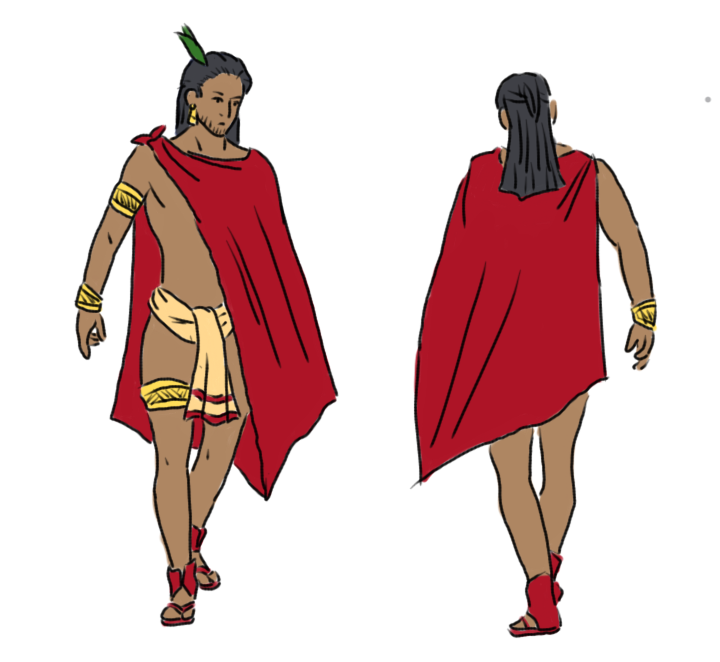
\includegraphics[height=0.3 \textheight]{Imagenes/tenelpan}
					\caption{Concepto de diseño de Tenépal.}
					\label{fig:tenelpanDiseno}
	\end{figure}
\subsection{Concepto:}
\begin{itemize}
	\item \textbf{Historia antes del juego:}
	Tenépal nació dentro de una familia noble y bien posicionada pero fue gracias a sus dotes como guerrero y a su gran carisma como líder que consiguió escalar socialmente hasta convertirse en el cacique de Oluta. Por consejo de su corte decide tomar por esposa a Cimatl, hermosa mujer de noble linaje que le permitió formar formar alianzas comerciales con diferentes pueblos de la región. Varios años despues de contraer nupcias, la pareja tuvo a su primera y única hija: Malinalli. 
	\\
	\par
	Durante los años venideros al nacimiento de su hija, Tenépal viajaría por distinto territorios del imperio, esto lo llevaría a concluir que la situación del imperio era demasiado frágil al no contar con una verdadera unión entre sus territorios, haciéndolo propicio de ser invadido por cualquier potencia con la suficiente astucia como para unir a los pueblos subyugados. En uno de sus viajes, Tenépal conoce a una sacerdotisa que clamaba ver el futuro, quien tras conocerlo le cuenta la profecía del legendario territorio conocido como el ombligo de la luna y como este sería el territorio que unificaría todos las culturas. Tras contarle la leyenda del ombligo de la luna, la sacerdotisa le asegura a Tenépal que su descendencia jugara un papel vital en la formación de este territorio. Es tras esta revelación que Tenépal decide iniciar su campaña para unificar los territorios del sur del imperio para iniciar una rebelión.
	\\
	\par
	La rebelión de Tenépal inicia como una conspiración secreta entre los gobernantes, los guerreros y la nobleza de los territorios sureños; sin embargo, todos los conspiradores son traicionados y mandados a ejecutar en secreto por el Tlatoani.  
	\item \textbf{Historia durante el juego:}
	Cuando el juego inicia Tenépal ya esta muerto, pero su recuerdo acompañara a Malianlli por toda su travesía, siendo su constante aliento y animo en los momentos difíciles.
	\item \textbf{Relaciones:}
	\begin{itemize}
		\item \textbf{Cimatl:} Esposa de Tenépal, ambos se casan por conveniencia sin poder formar un lazo emocional en los años que duraría su matrimonio. Su único punto en común es Malinalli, quien es a momentos utilizada por Cimatl para obtener lo que desea de su esposo (ver aparatado \ref{per:cimatl}).
		\item \textbf{Malinalli:} Hija de Tenépal, es la persona más importante en su vida y la persona a la que más ama. Tenépal cree totalmente en Malinalli (ver aparatado \ref{per:malinalli}). 
	\end{itemize}                     
\end{itemize}

\subsection{Encuentro:}
Aparece por primera vez en la cinemática 7 (ver aparatado \ref{Cin:Cinematica07}).
\subsection{Habilidades:}
Tiene las habilidades combativas de un un guerrero humano. Su principal habilidad es su capacidad de planear y de convencimiento.
\subsection{Armas:}
En sus años como guerrero usaba una Macuahuitl para enfrentarse a sus enemigos.
\subsection{Ítems:}
Sin ítems
\subsection{Bloques de animación}
\begin{itemize}
	\item Animación caminar.
	\item Animación normal.
\end{itemize}